%!TEX root = ../Master.tex
\chapter{Problem analysis}

\textit{In this chapter we will cover different problems associated with indoor navigation in a hospital. We will formulate our initiating problem, based on the issues that we relate to indoor navigation, and navigation in three dimensions. In the problem analysis we will work on the initiating problem, and delimit our initiating problem down to one problem statement, that we will try to solve.
}

\textbf{How can indoor navigation in hospitals be optimized by generating a specific route for individuals with different prerequisites?}

%!TEX root = ../../Master.tex
\section{Existing systems} % (fold)
\label{sec:existing_systems}


\paragraph{Phone}
Visitors are able to call the hospital's main number, and ask questions to a live operator. This can be done from any phone but there is no guarantee that a live operator is available.

\paragraph{Signs}
There are signs placed that mark different areas of the hospital. "Main entrance" and "Ambulance entrance" signs can be used to mark key places that the visitor can navigate from\cite{art_Osborne}.
Interior signs are also places in the hospital. These painted to the walls, affixed to doors or windows and others hanging from the ceiling. These describe what room or hall the visitor is in. Some of these signs also contain information about where the different areas of the hospital can be located, often marked by a line of text followed up by a arrow pointing in a specified direction. If the hospital is made up by multiple buildings, they can be numbered in order to navigate people to specific buildings.

\paragraph{Maps}
Maps offers a top-down view of the hospital with all the different locations marked by text or colour\cite{art_Osborne}. The map can be painted on a wall or found in a compact version meant to be carried around. The stationary maps often have a red dot that marks where the reader is. By knowing the current position, the visitor should be able to navigate with more ease as they won't have to look for something recognizable. If the building has multiple floors, the map will be split up into sections in order to cover all the rooms.

\paragraph{The receptionist}
The receptionist can answer questions from the visitors. Very much like the phone, but with some key differences. The phone is more accessible as the one calling does not need to be at the hospital. The receptions has an advantage of being more precise. There will be less confusion as body language can be used in the answering of the question.

\paragraph{Colour coding}
Coloured stripes across the wall or floor that leads to the different areas of the hospital. In the entrance hall the visitors will see a wall with some lines of text with a coloured stripe behind it. One line might say "recovery" and if followed, will lead to the recovery department. Some departments also have an entire theme in a certain colour. In this way, it might become easier for some people to navigate the next time they visit, if they can remember the colours representing the department. 

\paragraph{Porter}
The porter helps patients and visitors get around at the hospital. The porter helps visitors find available beds if they have to stay at the hospital overnight \cite{ugd_port}. 

% section existing_systems (end)

%!TEX root = ../../Master.tex
\section{Problems tied to the systems} % (fold)
\label{sec:Problems_tied_to_the_systems}

\paragraph{Phone}
The limitations regarding the phone, are high as the informer is limited by only having his/her voice as their tool. Miscommunication can occur as directions only can be delivered by words. As said before, this form for navigation strictly depends on a assigned personal to answer the phone. If no one is at the phone, it becomes utterly useless.
If the service is used often, more than one employee might be assigned to the phone. It could become an expensive service if there is a dedicated staff assigned to the phone. 

\paragraph{Signs}
The signs can be hard to spot if the  visitor is not familiar with the hospital, also a sign can be obstructed be other signs or if the room/hallway is filled with people. Another problem regarding the signs, is that might be hard to use if the visitor have reading problems. If the one who reads the sign can't understand the language or is an illiterate, it becomes hard to find the information that is relevant. To much information cn also be displayed on signs so that it becomes confusing or hard to see the system behind the sign placements.
Also, if the visitor is in building A, and wants to visit a patient in building B floor 6. It could become a challenge to set up enough signs to guide the visitor to the right building and floor, without drowning the other visitors with none relevant information.

\paragraph{Maps}
A big problem with maps is they can become very complicated to get a overview off if they cover multiple floors\cite{map_confusing}. If the visitor is already inside the building, t can sometimes be difficult to figure out where they are corresponding to the map. If they are standing in a hallway it can be difficult to distinguish it from the others. 

\paragraph{The receptionist}
If the visitor arrives at entrance different from the main one, they might not know where the receptionist is if they need help. The information received from the receptions have to be memorized when the visitor ventures away from the desk. This means that directions could become hard to remember if they have to get to distant location inside the building. A way the receptionist could help the visitor remember, would be to write a note but even so te text could be misunderstood or in other ways mixed up.

\paragraph{Colour coding}
If some rooms switches their function the stripes on the wall have to be repainted which will be a lot of work. If there stripes leading to all the different departments, a the information could potentially clutch up and become confusing. This method also shares a downside together with the signs, as people with reading disorder could have trouble with this form of navigation.

\paragraph{Porter}
The porter has other tasks he/she needs to attend to and will not always be available. Also, if the visitor have used the porter to get to a curtain room, and wants to leave an hour later, they might not know where to find a new one. 

% section Problems_tied_to_the_systems(end)

%\input{Chapters/problem_analysis/interessents_users.tex}
=======
%\input{Chapters/problem_analysis/interessents_users.tex}

%!TEX root = ../../Master.tex
\section{Leading Technologies}

http://www.wifarer.com/hospitals
http://www.meridianapps.com/products
http://www.smartindoor.com/
https://www.indooratlas.com/


\subsection{Position Technologies}

  \subsection{Satellites}

  \subsection{Cellular Communication Network}

  \subsection{Infra-red}

  \subsection{Blue-tooth}

  \subsection{WIFI}

  \subsection{Summary of Position Technologies}

\subsection{Positioning Techniques}

  \subsection{Cell of Origin}

  \subsection{Angle of Arrival}

  \subsection{Angle difference of Arrival}

  \subsection{Time of Arrival}

  \subsection{Time difference of Arrival}

  \subsection{Triangulation}

  Triangulation is a method used for estimating the position of an object. The method uses the properties of triangles. Triangulation has two derivatives: literation and angulation.

 \paragraph{Lateration}

  Lateration is commonly used technique for positioning.  Lateration uses the distance between known locations and and the point to be determined, to estimate the location.\cite{tri_lateration}  There are two types of lateration two dimensional and three dimensional. The two dimensional are use in robots that navigates in only one plane, like robot vacuum cleaners. 
  lateration in three dimensions are used in GPS positioning, and other practical applications for positioning.
  We will only explain three dimensional lateration.
  \begin{figure}[h!]
  \centering
  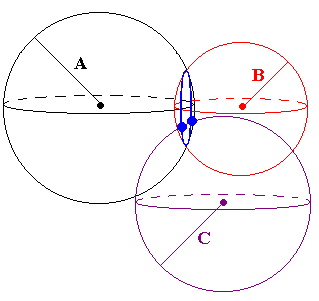
\includegraphics[width=3in]{trilateration}
  \caption{Example of lateration with three know positions.\newline Source: http://ixbtlabs.com/articles/gpssystem/}
  \label{fig:trilateration}
  \end{figure}
  

  Trilateration in three dimensions is possible in fare most situations if and only if the distance to three known positions is defined or possible to calculate.
  If we know a distance to one of these three positions we know that the point we are seeking is in the surface of a sphere, with center at the know position, and with a radius equals to the distance to the center. This is illustrated on figure \ref{fig:trilateration} as the surface of the sphere A.

  The intersection of two spheres is a circle. By determining the distance to a second know point it is possible to circumscribe the range of possible position to a smaller area.
  This is illustrated as the blue circle on figure \ref{fig:trilateration}, and is the intersection between sphere A and B.
  A third sphere that overlaps the intersection between the first two spheres, will mark 2 points where all three spheres is collapsing. In fare most situations there are only one of these locations that lies on the Earth's surface, the other point will often be fare in to the sky or deep inside earth. So by sorting one point from, there is only one possible position left. 
  In some very rare situation it is possible that both point lies on the Earth's surface, and in such situations the use of four spheres will determine witch of the to positions is the right one.



  \paragraph{Angulation}

  Angulation uses the technique called Angle of Arrival (AOA), which can compute the location of a source. The parameters needed are as minimum two relative angles between a remote point and the source, and the distance between the remote points. The source is at the location where the lines formed by the angle direction lines intercept. 

  In 2D, as few as two remote points are needed, given the source is not directly in between the remote points. However to improve accuracy and remove ambiguity, another remote point is needed. In 3D, as few as three remote points are needed. However as with 2D, another remote point improves accuracy and removes ambiguity. \cite{survey_pos, Sun2009, Boontrai2009}

  For example: rangers in location known fire lookout towers can use AOA to pinpoint where the fire is. See \cref{fig:aoa}. A ranger at tower A, sees the fire and notates the bearing to the fire. He then communicates with a ranger at tower B, telling him the general direction of the fire. The ranger at tower B now notates the bearing to the fire from his perspective. The fire can now be pinpointed from the 2 remote points (given the fire started in a 2-D world). The fire is where the 2 angle direction lines intercept. Ranger A at tower C can verify this position by also noting his bearing. \cite{compassdude_triangulation}

  \begin{figure}
    \centering
    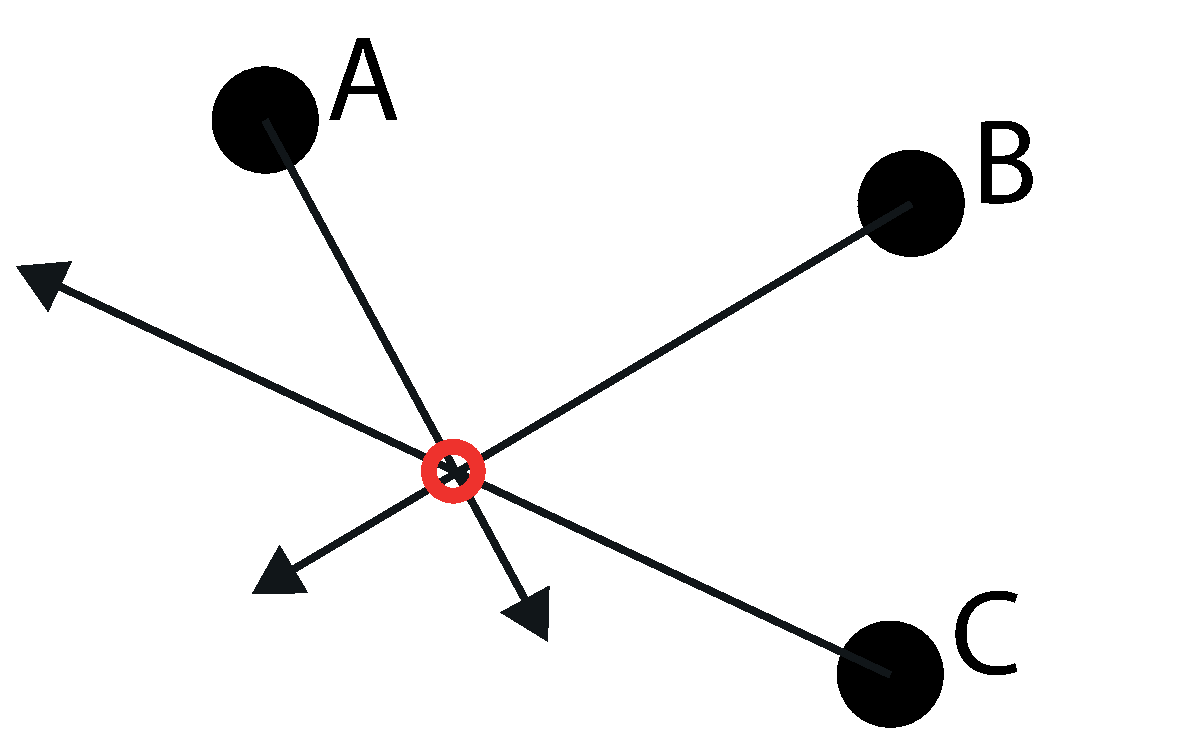
\includegraphics[width=\textwidth]{aoa.eps}
    \caption{Example of fire lookout towers positioning a fire using AOA.}
      \label{fig:aoa}
  \end{figure}

  The advantages of AOA are the few remote points needed in order to estimate a position. Another advantage is the independency of time synchronization.

  The disadvantages of AOA are the need of large and complex hardware requirements, and degradation of the location estimate as the target moves away from the measuring units. In order to perform accurate position of the target, very accurate angle measurements need to be performed. This can become a problem if the measuring is done in wireless networks, because of shadowing, multipath reflections arriving from misleading directions etc. Therefore angulation is best performed in free space.

  \subsection{Location Fingerprinting}

  \subsection{Summary of Position Techniques}

  \subsection{Information Techniques}

  \subsubsection{2 Dimensional map}

  \subsubsection{3 Dimensional map}

  \subsubsection{Text directions}

  \subsubsection{Summary of Information Techniques}

\subsection{Path finding Algorithms}

  Path finding algorithms is used for finding a path between to locations, the source and the destination. By searching its way from the source to the destination, until a path is found. These algorithms also make it possible to calculate the optimal path, I.e. the shortest.

  The algorithms to perform searches they makes use of a weighted graph. A graph, G is a set of nodes V, connected by links E.
  Information about destinations, rooms, entrances and exits would be represented as nodes and hallways and stairs would be represented as links. The distance to travel from node to node via a particular link, would be represented as a weight W(e).

  A important factor of a searching algorithm is correctness and also the time required to calculate the optimized path.
  The algorithms can be rated by their worst-case time, to ensure a responsive performance.


  %\begin{figure}[h!]
  %\caption{A picture of a gull.}
  %\centering
    %\includegraphics[width=0.5\textwidth]{/Images/pathfinding}
  %\end{figure}

  \paragraph{Dijkstra's Algorithm}

  A commonly used algorithm for finding the shortest path is Dijkstra's algorithm. Its loops through steps until all nodes to the target node is optimized with least cost, then points out the shortest path from source node, to target node. The need of every node being evaluated, the complexity of algorithm is proportional with the number of nodes, which means that a lot of computational power is required to calculate the result. The computational cost is calculated O(N*N), where N is the quantity of nodes in the graph.

  Another disadvantage with Dijkstra's algorithm is that its not possible to calculate negative weighted values, which could potentially cause the algorithm to engage in an infinite loop. A negative weighted value could mean saving money over loosing by passing through a certain area.

  We consider the problem: find shortest path from source to target.

  Where P is the source node, Q is the target and R is the evaluating node

  The nodes are subdivided into three sets:

  Set A - Optimized nodes (least costly path from P is known)
  Set B - Temporary nodes (evaluated cost of path from P but not part of set A)
  Set C - Remaining nodes

  The links are subdivided into three other sets:

  Set I - Links used in the set A
  Set II - Not part of set I (one and only one link of this set will lead to each node in set B)
  Set III - Remaining links (rejected or not yet considered)

  At first all nodes is assigned to set C and all links to set III, P is then assigned to set A.
  Then we loop through following steps until Q is part of set A.

  Step 1. Consider all the links r connecting the node just assigned to set A. If R is part of set C assign to set B and assign r to set II.
  If R is part of set B, then investigate if the use of link r is less costly from P to R than the existing link in set II. If less costly assign link r and reject existing link in set II, otherwise reject r to set III.

  Step 2. For each node in set B where there'Ps only one path in set I and set II, the node with minimum cost from P is assign to set A and with the corresponding link assign to set I.

  %\subsubsection{Bellman-Ford Algorithm}
%%%not relevant right now
  %is based on 3 separate algorithms


  \paragraph{A* Algorithm}

  Firstly A* is an informed search algorithm, where Dijkstra's is uninformed. A* utilises the principle of a heuristic estimation to determine which node to test next.

  - If h is zero, then only g affects the result and making it work like Dijkstra's algorithm

  - If h < g, the algorithm will guaranteed find the shortest path from source to target, at a slow running time.

  - If h == g, the algorithm will only extract the best path, but this not always possible due to obstacles.

  - If h > g, the algorithm will find a path fast not its not always the optimal.

  This means that the heuristic estimation should be reasonable, and not overestimate the distance between to the evaluating node and the target node. But should be just right for the final chosen path to be the optimal path and the for the complexity of the algorithm to be at a minimum.

  \paragraph{Summary of Algorithms}

  %SCHEME OF ADVANTAGES AND DISADVANTAGES
  %======================================
